\documentclass[12pt,3p]{article}
\usepackage[margin=0.75in]{geometry}

\usepackage[T1]{fontenc}
\usepackage[utf8]{inputenc}
\usepackage[english]{babel}
\usepackage{amsmath}
\usepackage{mathtools}
\usepackage{enumitem}
\usepackage{physics}
\usepackage{bm}
\usepackage[round,numbers]{natbib}
\usepackage[font=small]{caption}

\usepackage[colorlinks = false]{hyperref}

\begin{document}

\title{\Large{Hertzian Contact with a Rigid Indenter Using a Penalty Approach} \vspace{-2ex}}
\author{Ida Ang (Edited \today)}
\date{\vspace{-5ex}}
\maketitle

\tableofcontents
\newpage

\section{Problem Definition}
\vspace{-2ex}
Formulation of frictionless contact between the rigid surface (indenter) and an elastic domain, representing an infinite half-space. The elastic domain is approximated using a linear elastic isotropic constitutive relationship. Contact will be solved using a penalty formulation allowing a small amount of interpenetration between the solid and the indenter. The penalty method is a non-exact method of contact. 

\subsection{Weak Form}
Starting from the equilibrium equation:
\begin{equation}
- \text{Div} \bm{\sigma} = \bm{f} \rightarrow - \div \bm{\sigma} = \bm{f} 
\end{equation}
Write in indicial and convert to weak form 
\begin{align}\label{befIntParts}
\begin{split}
- \pdv{\sigma_{ij}}{x_j} \mathbf{e_i} &= f_k \mathbf{e_k} \quad \text{Multiply by a test function} \\
-\pdv{\sigma_{ij}}{x_j} \mathbf{e_i} \cdot v_p \mathbf{e_p} &= f_k \mathbf{e_k} \cdot v_p \mathbf{e_p} \\
-\pdv{\sigma_{ij}}{x_j} v_p \delta_{ip} &= f_k v_p \delta_{kp} \\
-\pdv{\sigma_{ij}}{x_j} v_i &= f_k v_k \quad \text{Integrate over the domain} \\
-\int_{\Omega_o} \pdv{\sigma_{ij}}{x_j} v_i dV &= \int_{\Omega_o} f_k v_k dV
\end{split}
\end{align}
Integration by parts on the left hand side of Eq. \ref{befIntParts}
\begin{align*}
(fg)' = f'g + fg' \rightarrow f'g &= (fg)' - fg' \\
\pdv{\sigma_{ij}}{x_j} v_i &= (\sigma_{ij} v_i)_{,j} - \sigma_{ij} \pdv{v_i}{x_j}
\end{align*}
Substitute this into Eq. \ref{befIntParts}
\begin{align*}
-\int_{\Omega_o}  (\sigma_{ij} v_i)_{,j} dV + \int_{\Omega_o} \sigma_{ij} \pdv{v_i}{x_j} dV &= \int_{\Omega_o} f_k v_k dV \quad \text{Use the divergence theorem} \\
-\int_{\partial \Omega_o} \sigma_{ij} v_i n_j dS + \int_{\Omega_o} \sigma_{ij} \pdv{v_i}{x_j} dV &= \int_{\Omega_o} f_k v_k dV \quad \text{Recognize the traction term} \\
-\int_{\partial \Omega_o} t_i v_i dS + \int_{\Omega_o} \sigma_{ij} \pdv{v_i}{x_j} dV &= \int_{\Omega_o} f_k v_k dV \quad \text{Rearrange}\\
 \int_{\Omega_o} \sigma_{ij} \pdv{v_i}{x_j}  dV &= \int_{\Omega_o} f_k v_k dV + \int_{\partial \Omega_o} t_i v_i dS
\end{align*}
The principle of virtual work states that:
\begin{equation}\label{PVW}
\int_{\Omega} b_i \delta u_i dV + \int_{\partial \Omega} t_i \delta u_i dS  = \int_{\Omega} \sigma_{ij} \delta \epsilon_{ij} dV = \int_{V} \delta W dV
\end{equation}
Applying this principle to the LHS of our equation where f is equivalent to the body force, b:
\begin{align}\label{tempWF}
\begin{split}
\int_{\Omega_o} \sigma_{ij} \pdv{v_i}{x_j}  dV = \int_{\Omega_o} f_k v_k dV + \int_{\partial \Omega_o} t_i v_i dS &= \int_{\Omega} \sigma_{ij}  \epsilon_{ij} dV \quad \text{No traction or body forces} \\
0 &= \int_{\Omega} \sigma_{ij}  \epsilon_{ij} \, dV 
 \end{split}
\end{align}
In direct notation, 
\begin{equation}
\int_{\Omega} \bm{ \sigma(u) : \bm{\epsilon(v) }} \, d \Omega = 0 
\end{equation}


\subsection{Strain Energy Density}
The strain energy density can be defined with the following equation,
\begin{align*}
\Psi = \lambda \tr{\bm{\epsilon}} \mathbf{I} + 2 \mu \bm{\epsilon}
\end{align*}
where the elasticity parameters are defined as the shear modulus, $\mu$ (Lame's second parameter) and Lame's first parameter $\lambda$. Note that {\fontfamily{qcr}\selectfont lambda} is a keyword in FEniCS so we define {\fontfamily{qcr}\selectfont lmbda}. \\
{\fontfamily{qcr}\selectfont
E, nu = 10.0, 0.3 \\
mu = Constant(E/(2*(1 + nu))) \\
lmbda = Constant(E*nu/((1 + nu)*(1 - 2*nu))) \\ 
}
where E is the elasticity modulus and $\nu$ is Poisson's ratio, a measure of incompressibility. 

\section{Contact Formulation}
\vspace{-2ex}
The rigid indenter with a spherical surface can be approximated by a parobolic equation instead of explicitly modeled and meshed. Consider the indenter radius, R, to be sufficiently large with respect to the contact region characteristic size ($R >> a$). This relationship, $R > > a$, allows the spherical surface to be approximated by a parabola. 
\begin{equation}\label{indenter}
h(x,y) = -h_o + \frac{1}{2R} (x^2 + y^2)
\end{equation}
where $h_o$ is the initial gap between both surfaces at x = y = 0 (the center of the indenter). 
 
 The unilateral contact condition on the top surface $\Gamma$ is known as the Hertz-Signorini-Moreau conditions for frictionless contact 
\begin{equation}
g \geq 0, \quad p \leq 0, \quad g \cdot p = 0 \quad \text{on } \Gamma
\end{equation}
The gap, $g$, is defined as follows,
\begin{equation*}
g = u_z - h(x,y)
\end{equation*}
where we specify the displacement $u_z$, which indicates only normal contact is considered. $p = - \sigma_{zz}$ is the pressure. 

\subsection{Penalty Approach}
The penalty approach is an inexact method, dependent on the magnitude of a constant known as the penalty parameter. The simplest way to solve this contact condition is to replace the previous complementary conditions by the following penalized condition:
\begin{align}\label{penalty}
\begin{split}
p &= k_{pen} \langle g \rangle_{+} \quad \text{where } g = u_z - h(x,y)  \\
	&= k_{pen} \langle u_z - h(x,y) \rangle_{+}
\end{split}
\end{align}
where $k_{pen}$ is a large penalizing stiffness coefficient, and we have the definition of the Mackauley bracket
\begin{equation}\label{ppos}
\langle x \rangle_{+} = \frac{|x| + x}{2} 
\end{equation}
Therefore, we can add the penalty term in Eq. \ref{penalty} to Eq. \ref{tempWF} after multiplying by the test function 
\begin{equation*}
\int_{\Omega} \bm{ \sigma(u) : \bm{\epsilon(v) }} \, d \Omega + k_{pen} \int_{\Gamma} \langle g \rangle_{+} v_z \, dS  = 0 
\end{equation*}
where it is important to note that $dS$ represents the top surface that will experience contact. 

An illustration of how the penalty formulation works is demonstrated in Fig. \ref{FigPenaltyVarying}. A too high penalty parameter can lead to ill-conditioning of the stiffness matrix, but also correlates to better contact enforcement. As the penalty parameter increases, the gap function is more closely enforced at 0, resulting in a displacement that matches the indenter.

\begin{figure*}[!htb]
\centering
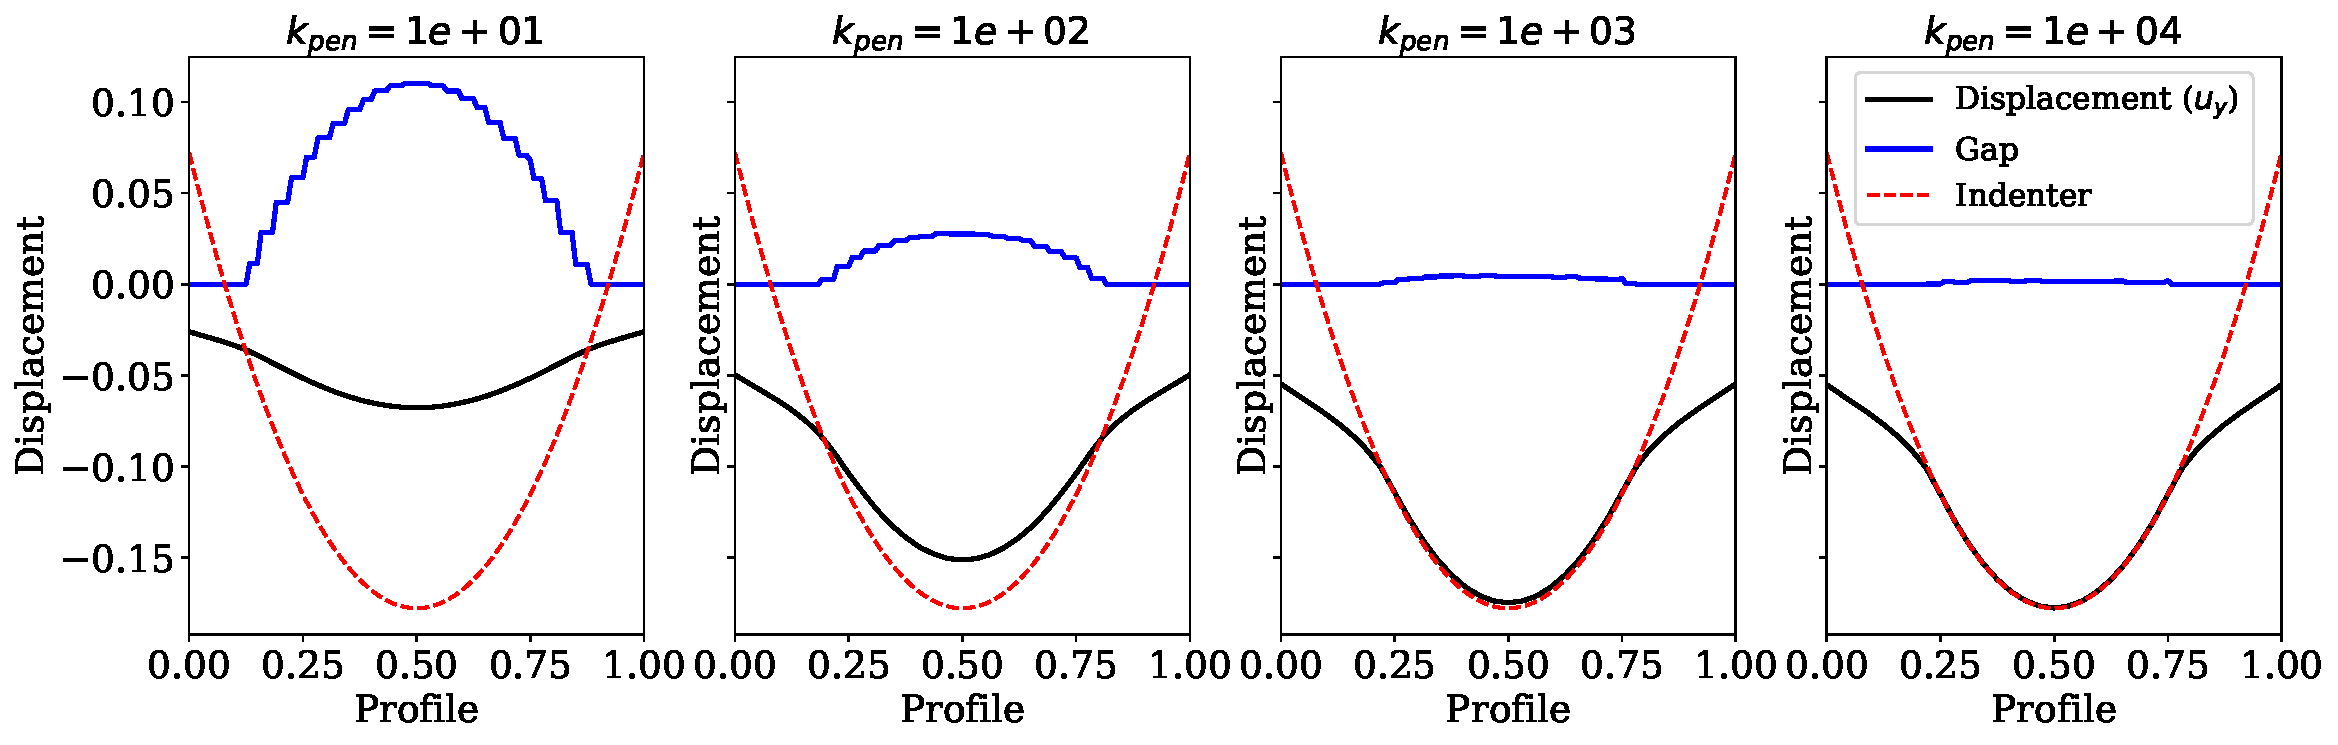
\includegraphics[width=\textwidth]{./Images/PenaltyVarying.pdf}
\caption{Displacement in the downwards direction $u_y$ in black, gap function in blue, and indenter in red alongside the top surface. The same amount of contact is enforced in each case, as represented by the same indenter profile, where the penalty parameter is varying from a low to high value.}
\label{FigPenaltyVarying}
\end{figure*}


\section{FEniCS Implementation}
\vspace{-2ex}
FEniCS implementation was originally provided in 3D, and changes were made to simplify the problem into a 2D problem. 

\subsection{Analytical Solution}
The analytical problem gives the following: 
\begin{itemize}
\item The contact area, a, is of circular shape (d = depth) and radius, R.
	\begin{equation*}
	a = \sqrt{Rd}
	\end{equation*}
\item The force exerted by the indenter onto the surface is:
	\begin{equation*}
	F = \frac{4}{3} \frac{E}{(1+ \nu^2)} ad
	\end{equation*}
\item The pressure distribution on the contact region is given by ($p_o$ is the maximal pressure):
	\begin{equation*}
	p(r) = p_o \sqrt{1 - (\frac{r}{a})^2} \quad \quad p_o = \frac{3F}{2 \pi a^2}
	\end{equation*}
\end{itemize}
These can be solved for in FEniCS \\
{\fontfamily{qcr}\selectfont
a = sqrt(R*d) \\
F = 4/3.*float(E)/(1-float(nu)**2)*a*d \\
p0 = 3*F/(2*pi*a**2) \\ \\
}
Print the maximum pressure and applied force \\
{\fontfamily{qcr}\selectfont
print("Maximum pressure FE: \{0:8.5f\} Hertz: \{1:8.5f\}" \\
\indent \indent.format(max(np.abs(p.vector().get\_local())), p0)) \\
print("Applied force FE: \{0:8.5f\} Hertz: \{1:8.5f\}" \\
\indent \indent .format(4*assemble(p*ds(1)), F)) \\ \\
}

%Refine the mesh size to a smaller size closer to the contact area (x = y = z = 0). The indexing [:, :2] refers to the x and y directions where this specifies 0 and 1 \\
%{\fontfamily{qcr}\selectfont
%mesh.coordinates()[:, :2] = mesh.coordinates()[:, :2]**2 \\ \\
%}
%Refine the mesh where indexing [:,2] refers to the z direction. Use a negative sign to indicate downwards from the point of contact at (x = y = z = 0) \\
%{\fontfamily{qcr}\selectfont
%mesh.coordinates()[:, 2] = -mesh.coordinates()[:, 2]**2 \\ \\
%}
\end{document}
